\chapter{强耦合常数 $\alpha_s$}

谱学研究除了检验 QCD 之外，还允许确定标准模型的一些基本参数，即耦合常数 $\alpha_s$ 和夸克质量。要确定 $\alpha_s$，不仅需要知道它的强度，还需要知道测量该耦合常数的能量标度 $Q$。一般而言，$\alpha_s$ 的计算过程如下。人们选取一个能够被非常精确测量的量 $O$，无论是在高能实验中还是在格点上通过非微扰方法测量，并且已知其微扰展开，即
\begin{equation}
O = \sum_n A_n \alpha_s^n(Q),
\end{equation}
其中 $A_n$ 是微扰系数。对该关系求逆即可得到 $\alpha_s(Q)$。

一种有前景的计算 $\alpha_s$ 的格点方法由 NRQCD 合作组开创 [110]。他们考察若干短距离量 $O$，例如小威尔逊圈的期望值，这些量可以在格点上被非常精确地计算，并且其微扰展开至少已知到 $O(\alpha_s^2)$ 阶。表征这些格点可观测量能量的标度 $Q$ 通常具有 $Q = C/a$ 的形式，其中 $a$ 是格距，$C$ 是一个需要确定的常数。他们通过评估这些量微扰表达式中的平均动量流来确定与 $O$ 相关的常数 $C$。标度 $1/a$ 利用夸克偶素的能级劈裂来固定。具体而言，他们使用 Upsilon 系统中自旋平均的 S-P 劈裂和 1S-2S 劈裂。使用这些劈裂的优点是，它们对底夸克质量的精细调谐几乎不敏感，并且轻夸克圈带来的修正预计很小。

最后，为了将格点方案中的 $\alpha_s$ 转换到 $\alpha_{\overline{\mathrm{MS}}}$，他们使用两圈关系，并在误差分析中纳入对 $\alpha_s^3$ 项的合理估计。他们的最终估计
\begin{equation}
\alpha_{\overline{\mathrm{MS}}}(M_Z) = 0.1174(24)
\end{equation}
包含了淬火不确定度。这一异常精确的结果与实验测定的世界平均值 $\alpha_s = 0.118(3)$ 一致，如图~\ref{fig:33} 所示。

ALPHA 合作组采用了一种测量 $\alpha_s$ 的替代方法 [182]。在他们称为薛定谔泛函方法的方法中，$\alpha_s$ 通过测量格点系统对外场的响应来定义。他们利用某个固定距离（$R_0 = 0.5$ 费米）处的力来固定格点标度 $a$。他们使用非微扰重整化群步进过程将其耦合演化到非常高的标度。在此高标度下，他们用两圈关系定义 $\Lambda^{(0)}_{\overline{\mathrm{MS}}}$，并在误差估计中纳入（很小的）三圈不确定度。他们已经完成了淬火理论的这一计算，得到结果 $\Lambda^{(0)}_{\overline{\mathrm{MS}}} = 251(21)$~MeV，目前正在进行 $n_f = 2$ 的模拟 [182]。相应的值 $\alpha_{\overline{\mathrm{MS}}}(90~\mathrm{GeV}) = 0.0818(10)$ 低于自然界中的值。这一差异被归因于忽略了海夸克效应。

\begin{figure}[htbp]
\centering
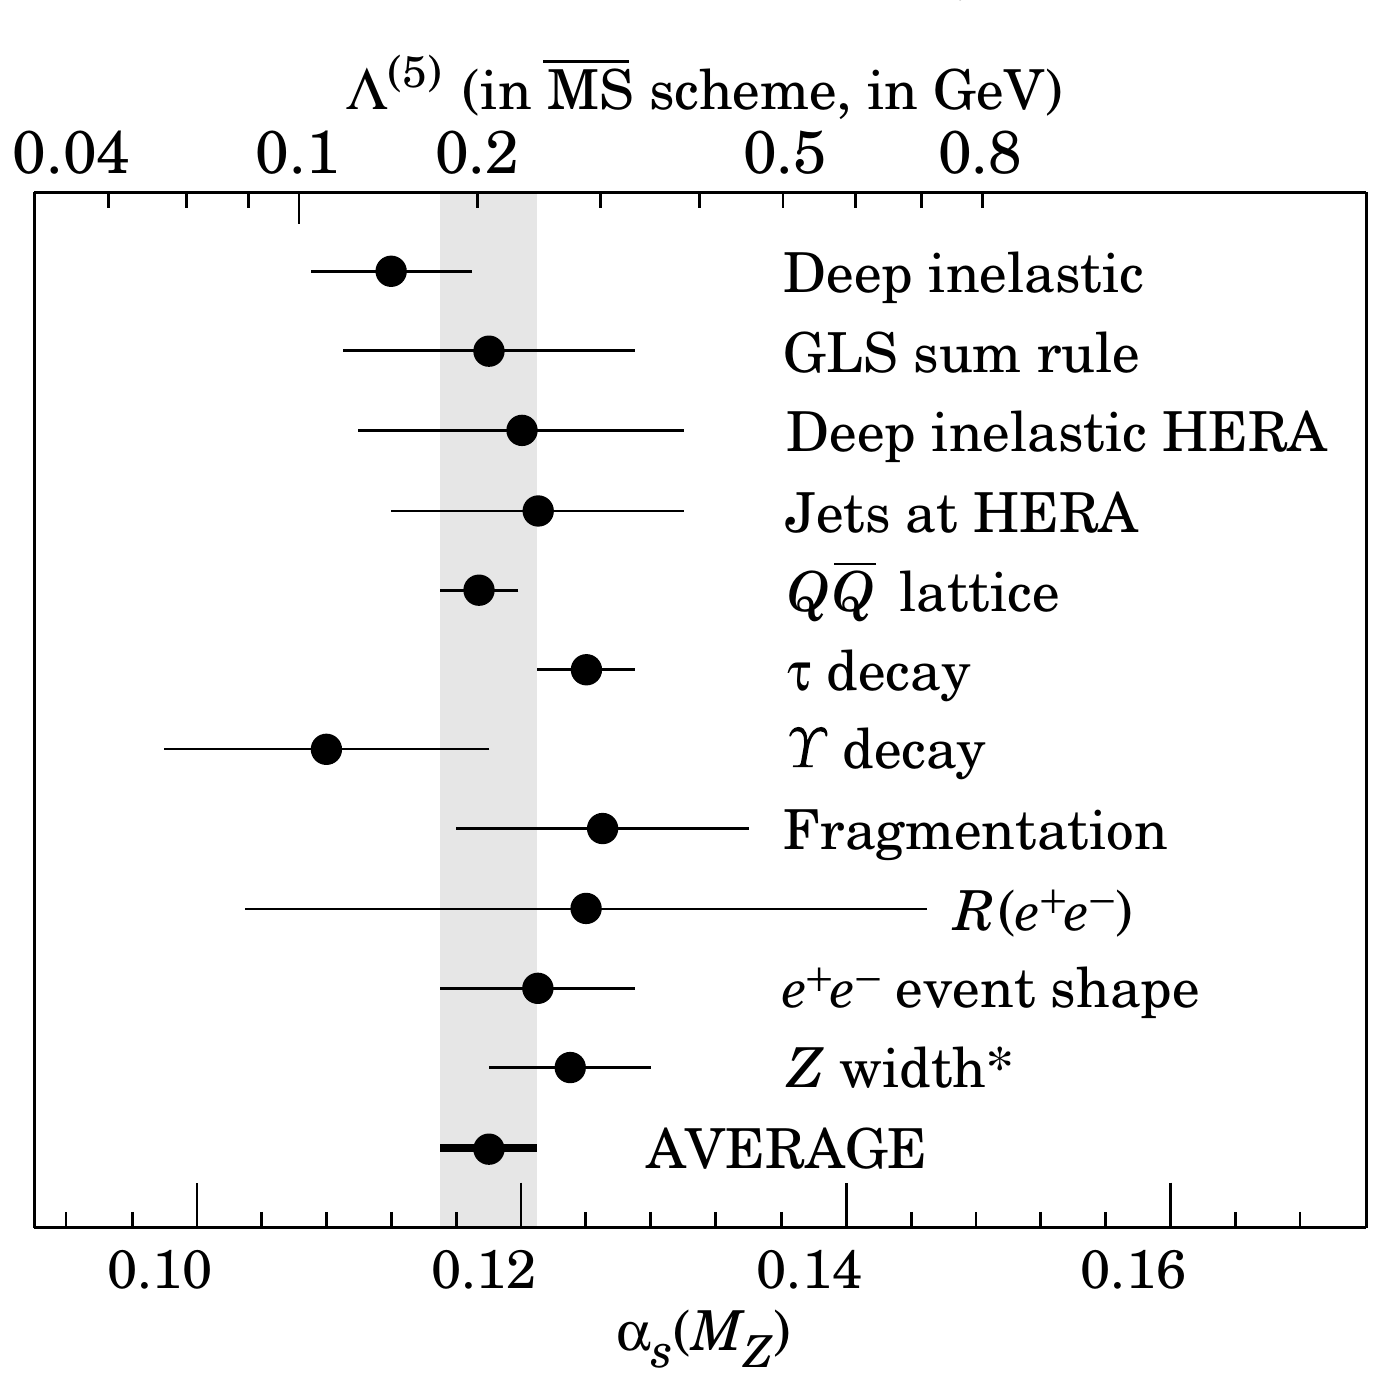
\includegraphics[width=0.8\textwidth]{images/fig33.png}
\caption{从各种过程中提取的 $\alpha_s(M_Z)$ 与 $\Lambda^{(5)}$（5 种活跃夸克味对应的 QCD 标度）数值的汇总。这些结果按测量能量标度的升高自上而下排列。此图复制自 1996 年《粒子物理评论》（Review of Particle Physics），并更新以显示最新的格点结果 $\alpha_{\overline{\mathrm{MS}}}(M_Z) = 0.1174 \pm 0.0024$。从不同标度的过程中提取的 $\alpha_s$ 具有相同的数值，这是对 QCD 的一个显著验证。}
\label{fig:33}
\end{figure}

如果不对淬火近似做任何修正，NRQCD 分析也会得到类似的偏低数值。关于薛定谔泛函方法的细节，参见吕舍尔（Lüscher）教授在本学校的讲义。
